% Local proposal only. Original palette and IEEEtran serif typography retained.
% Photo is the existing scene crop; the adjacent coupling diagram is schematic.
\definecolor{jepa}{HTML}{2A78D6}
\definecolor{war}{HTML}{EB6834}
\definecolor{pets}{HTML}{1BAF7A}
\definecolor{refgrey}{HTML}{8A8984}
\definecolor{ink}{HTML}{0B0B0B}
\definecolor{inktwo}{HTML}{52514E}
\definecolor{rule}{HTML}{D3D1C7}
\definecolor{panel}{HTML}{F7F6F3}
\definecolor{banner}{HTML}{ECEBE7}
\definecolor{probe}{HTML}{6250D6}
\begin{tikzpicture}[
  font=\fontsize{8}{9.2}\selectfont, >={Stealth[length=4pt,width=3.5pt]},
  panel/.style={draw=rule,fill=panel,rounded corners=4pt,line width=.5pt},
  heading/.style={font=\fontsize{8}{9.2}\selectfont\bfseries,text=ink,anchor=north west,inner sep=0pt},
  note/.style={font=\fontsize{7.3}{8.5}\selectfont,text=inktwo,inner sep=1pt},
  chip/.style={draw=#1,fill=#1!12,rounded corners=2pt,line width=.6pt,
    text width=3.78cm,font=\fontsize{7}{8.3}\selectfont,align=left,inner xsep=4pt,inner ysep=4pt,anchor=west},
  stage/.style={draw=inktwo,fill=white,rounded corners=2pt,line width=.5pt,
    minimum height=.5cm,text width=3.3cm,align=center,font=\fontsize{8}{9.2}\selectfont\mdseries},
  slot/.style={stage,draw=ink,dash pattern=on 3pt off 1.5pt,line width=.9pt,
    minimum height=.62cm,font=\fontsize{8}{9.2}\selectfont\bfseries},
  flow/.style={->,draw=inktwo,line width=.6pt},
  real/.style={->,draw=ink,line width=.9pt},
  effect/.style={->,draw=probe,line width=.9pt},
  probe/.style={circle,fill=probe,text=white,inner sep=0pt,minimum size=.36cm,font=\tiny\bfseries},
  card/.style={draw=rule,fill=white,rounded corners=3pt,line width=.5pt}
]
\fill[banner,rounded corners=4pt] (0,7.25) rectangle (18,7.85);
\node[font=\small\bfseries,text=ink] at (9,7.55) {Does a model that predicts well also fly well?};

% Replace the predictor; retain the common planner, cost and task.
\draw[panel] (0,2.85) rectangle (4.35,7.05);
\node[heading] at (.15,6.91) {Replace: the predictor};
\node[chip=jepa] at (.15,6.18)
  {JEPA: \texttt{full}, \texttt{no\_cross}, \texttt{flat}\\[2pt]
   Cross-agent information flow};
\node[chip=war] at (.15,5.35) {W-ar: autoregressive state model};
\node[chip=pets] at (.15,4.70) {PETS: probabilistic ensemble};
\node[note,anchor=west] at (.15,4.04) {Physics references};
\node[chip=refgrey] at (.15,3.57)
  {fixed / estimated load mass};

\draw[panel] (4.75,2.85) rectangle (9.6,7.05);
\node[heading,font=\fontsize{7}{8.3}\selectfont\bfseries] at (4.90,6.91) {Keep fixed: MPPI planner and shared cost};
\node[stage] (cand) at (6.90,6.18) {candidate plans};
\node[slot] (wm) at (6.90,5.28) {world model under test};
\node[stage] (fut) at (6.90,4.38) {predicted futures};
\node[stage] (pick) at (6.90,3.48) {cost-weighted plan};
\draw[flow] (cand)--(wm);
\draw[flow] (wm)--(fut);
\draw[flow] (fut)--(pick);
\draw[real] (4.35,5.28)--(wm.west);

% Existing scene plus a schematic of influence transmitted through the load.
\draw[panel] (10.00,2.85) rectangle (18,7.05);
\node[heading] at (10.15,6.91) {Test: shared-load transport};
\draw[card] (10.15,3.05) rectangle (15.05,6.52);
\draw[card] (15.25,3.05) rectangle (17.85,6.52);
\node[heading,font=\fontsize{7.5}{8.5}\selectfont\bfseries] at (10.30,6.37) {Task scene};
\node[heading,font=\fontsize{7.5}{8.5}\selectfont\bfseries] at (15.40,6.37) {Cross-agent effect};
\node[anchor=north west,inner sep=0pt] (scene) at (10.60,5.99)
  {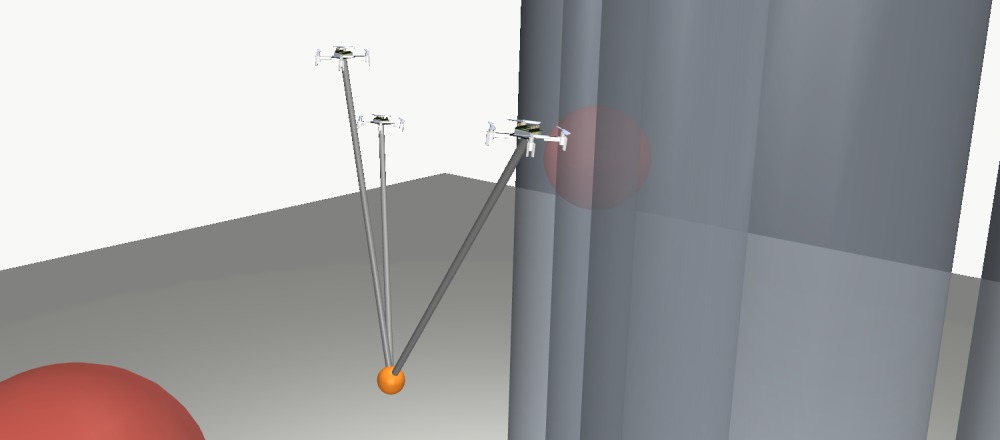
\includegraphics[width=4.00cm]{approved_figures_20261105/teaser_task_crop.png}};
\draw[rule,line width=.5pt] (scene.south west) rectangle (scene.north east);
\node[note,anchor=north west,text width=4.00cm,inner sep=0pt,font=\fontsize{7}{8.3}\selectfont] at (10.60,4.05)
  {Three UAVs carry one load\\[2pt]
   Hidden mass and state delay\\[2pt]
   Static and moving obstacles};
\coordinate (A) at (16.55,5.82);
\coordinate (B) at (15.80,5.30);
\coordinate (C) at (17.25,5.30);
\coordinate (load) at (16.55,4.65);
\foreach \p in {A,B,C} {
  \draw[refgrey,line width=.65pt] (\p)--(load);
  \draw[ink,line width=.7pt] ([xshift=-.15cm]\p)--([xshift=.15cm]\p);
  \draw[ink,line width=.7pt] ([yshift=-.10cm]\p)--([yshift=.10cm]\p);
  \fill[ink] (\p) circle (.045cm);
}
\fill[ink] (load) circle (.085cm);
\node[note,anchor=west] at (16.71,5.82) {A};
\node[note,anchor=east] at (15.64,5.30) {B};
\node[note,anchor=west] at (17.41,5.30) {C};
\node[note,anchor=north] at (16.55,4.46) {load};
\draw[effect] (16.63,5.66)--(16.63,4.87);
\draw[effect] (16.38,4.74)--(15.93,5.13);
\draw[effect] (16.73,4.74)--(17.12,5.13);
\node[note,anchor=north west,text width=2.26cm,inner sep=0pt,font=\fontsize{7}{8.3}\selectfont] at (15.42,4.05)
  {Change A's plan.\\[2pt]
   Predict the response\\[2pt]
   of load and B/C.};

% Real closed loop: state feedback and executed setpoints have distinct paths.
\draw[real] (10.00,6.18)--(cand.east);
\node[note,anchor=south,align=center,font=\fontsize{6}{7}\selectfont] at (9.30,6.23) {delayed\\state};
\draw[real] (pick.east)--(10.00,3.48);
\node[note,anchor=south,align=center,font=\fontsize{6}{7}\selectfont] at (9.30,3.53) {execute\\setpoints};

% Four complementary views, rather than repeating the metric diagrams in Fig.4.
\draw[panel] (0,0) rectangle (18,2.62);
\node[heading] at (.15,2.48) {Measure: from prediction to mission success};
\draw[card,draw=inktwo,line width=.65pt] (10.50,2.12) rectangle (17.85,2.51);
\node[note,font=\fontsize{7}{8}\selectfont] at (14.17,2.315)
  {Oracle U: exact simulator references for layers 1--3};
\foreach \x/\n/\name/\text in {
  .15/1/Prediction/{Same plan, future load},
  4.65/2/Counterfactual/{Changed plan, cross-agent response},
  9.15/3/Decision/{Executed plan, true regret},
  13.65/4/Mission/{Closed-loop flight, success $J$}} {
  \draw[card] (\x,1.11) rectangle ++(4.20,.85);
  \node[probe] at (\x+.28,1.67) {\n};
  \node[anchor=west,font=\fontsize{8}{9.2}\selectfont\bfseries,inner sep=0pt]
    at (\x+.53,1.67) {\name};
  \node[note,anchor=west,font=\fontsize{7}{8}\selectfont,inner sep=0pt]
    at (\x+.15,1.30) {\text};
}
\draw[card,draw=probe,line width=.8pt] (.15,.16) rectangle (17.85,.87);
\node[anchor=west,font=\fontsize{8}{9.2}\selectfont\bfseries,inner sep=0pt,text=ink] at (.32,.51)
  {Pre-registered test};
\node[note,anchor=west,font=\fontsize{8}{9.2}\selectfont,inner sep=0pt] at (3.53,.51)
  {Does cross-agent error $L_2$ add information about success $J$ beyond trajectory error $L_1$?};
\end{tikzpicture}
